%%%%%%%%%%%%%%%%%%%%%%%%%%%%%%%%%%%%%%%%%
% Short Sectioned Assignment
% LaTeX Template
% Version 1.0 (5/5/12)
%
% This template has been downloaded from:
% http://www.LaTeXTemplates.com
%
% Original author:
% Frits Wenneker (http://www.howtotex.com)
%
% License:
% CC BY-NC-SA 3.0 (http://creativecommons.org/licenses/by-nc-sa/3.0/)
%
%%%%%%%%%%%%%%%%%%%%%%%%%%%%%%%%%%%%%%%%%

%----------------------------------------------------------------------------------------
%	PACKAGES AND OTHER DOCUMENT CONFIGURATIONS
%----------------------------------------------------------------------------------------

\documentclass[paper=a4, fontsize=11pt]{scrartcl} % A4 paper and 11pt font size

\usepackage[T1]{fontenc} % Use 8-bit encoding that has 256 glyphs
\usepackage{fourier} % Use the Adobe Utopia font for the document - comment this line to return to the LaTeX default
\usepackage[english]{babel} % English language/hyphenation
\usepackage{amsmath,amsfonts,amsthm} % Math packages
\usepackage{graphicx}
\usepackage{lipsum} % Used for inserting dummy 'Lorem ipsum' text into the template

\usepackage{sectsty} % Allows customizing section commands
\allsectionsfont{\centering \normalfont\scshape} % Make all sections centered, the default font and small caps

\usepackage{fancyhdr} % Custom headers and footers
\pagestyle{fancyplain} % Makes all pages in the document conform to the custom headers and footers
\fancyhead{} % No page header - if you want one, create it in the same way as the footers below
\fancyfoot[L]{} % Empty left footer
\fancyfoot[C]{} % Empty center footer
\fancyfoot[R]{\thepage} % Page numbering for right footer
\renewcommand{\headrulewidth}{0pt} % Remove header underlines
\renewcommand{\footrulewidth}{0pt} % Remove footer underlines
\setlength{\headheight}{13.6pt} % Customize the height of the header

\numberwithin{equation}{section} % Number equations within sections (i.e. 1.1, 1.2, 2.1, 2.2 instead of 1, 2, 3, 4)
\numberwithin{figure}{section} % Number figures within sections (i.e. 1.1, 1.2, 2.1, 2.2 instead of 1, 2, 3, 4)
\numberwithin{table}{section} % Number tables within sections (i.e. 1.1, 1.2, 2.1, 2.2 instead of 1, 2, 3, 4)

\setlength\parindent{0pt} % Removes all indentation from paragraphs - comment this line for an assignment with lots of text

%----------------------------------------------------------------------------------------
%	TITLE SECTION
%----------------------------------------------------------------------------------------

\newcommand{\horrule}[1]{\rule{\linewidth}{#1}} % Create horizontal rule command with 1 argument of height

\title{	
\normalfont \normalsize 
\textsc{University of California, Los Angeles\\
Department of Computer Science} \\ [25pt] % Your university, school and/or department name(s)
\horrule{0.5pt} \\[0.4cm] % Thin top horizontal rule
\huge CS 276A assignment 1 \\ % The assignment title
\horrule{2pt} \\[0.5cm] % Thick bottom horizontal rule
}

\author{Yang Pei\\
304434922} % Your name

\date{\normalsize\today} % Today's date or a custom date

\begin{document}

\maketitle % Print the title

%----------------------------------------------------------------------------------------
%	PROBLEM 1
%----------------------------------------------------------------------------------------

\section{Problem 1}

\begin{enumerate}
\item Since we use a Bayes decision for $\alpha(x)$, according to the textbook, we can use $g_{i}(x) = -R(\alpha_{i}|x)$ as our discriminant function, which is given by:
\begin{equation}
R(\alpha_{i}|x) = \sum_{j=1}^{c}\lambda(\alpha_{i}|\omega_{j})p(\omega_{j}|x)
\end{equation}
The risk matrix is given and all we need to do is to calculate the posterior probability which is given by:
\begin{equation}
p(\omega_{j}|x) = p(x|\omega_{j})*p(\omega_{j})
\end{equation}
Here we have omit the component $p(x)$ since it is only a scale factor. The $p(x|\omega_{j})$ is given and all are mulit norm distribution with the covariance matrixs all the same, so we can omit the term $\frac{1}{(2\pi)^{d/2}|\Sigma|^{1/2}}$ and this would not effect our discriminant functions. Combine the information above, the final discriminant for each category are:
\begin{equation}
\begin{aligned}
g_{1} = -1.2*e^{-1/18*[(x_{1} - 12)^{2}+(x_{2} - 3)^{2}]} -0.4*e^{-1/18*[(x_{1} - 3)^{2}+(x_{2} - 5)^{2}]}\\
g_{2} = -0.8*e^{-1/18*[(x_{1} - 4)^{2}+(x_{2} - 12)^{2}]} -0.2*e^{-1/18*[(x_{1} - 3)^{2}+(x_{2} - 5)^{2}]}\\
g_{3} = -1.2*e^{-1/18*[(x_{1} - 4)^{2}+(x_{2} - 12)^{2}]} -0.4*e^{-1/18*[(x_{1} - 12)^{2}+(x_{2} - 3)^{2}]}
\end{aligned}
\end{equation}

\item The decision boundaries for each two categories are shown in figure \ref{fig:1}.
\begin{figure}[htbp]
	\centering
		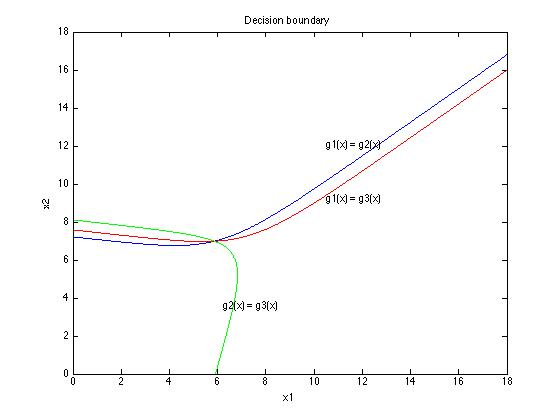
\includegraphics[width = 5in]{figure1.jpg}
		\caption{Decision boundaries}
		\label{fig:1}
		
		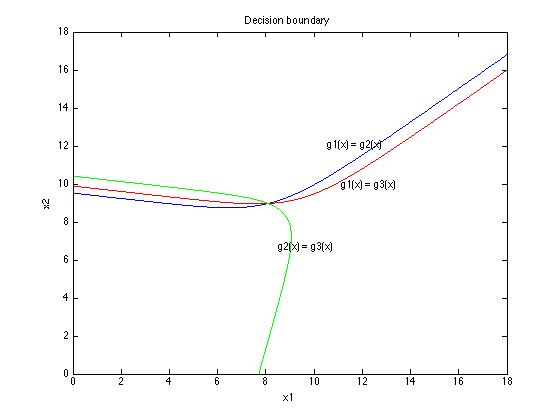
\includegraphics[width = 5in]{figure2.jpg}
		\caption{New decision boundaries}
		\label{fig:2}
\end{figure}

\item Given the new prior distribution, the new decision boundaries for each two categories are shown in figure \ref{fig:2}. We could see that the shape does not have too much change, but it is shfit from left to right due to a higher prior distribution for category 3.
\end{enumerate}
%------------------------------------------------
%	PROBLEM 2
%----------------------------------------------------------------------------------------

\section{Problem 2}

%------------------------------------------------
\begin{enumerate}
\item The average risk is computed as 
\begin{equation}
R = \int R(\alpha(x)|x)p(x)dx
\end{equation}
where $\alpha(x)$ is the decision function which maps an input to an action. In Bayes decision, we always map to the action, or decision, with the largest posterior probability $$\alpha_{Bayes}(x) = y^{*} = arg\max\limits_{y\in\Omega^{c}}p(y|x) $$
and this is determined. In terms of randomized decision rule, the action is not determined, which is given by $$\alpha_{ran}(x) = y \sim p(y|x)$$
In order to compute the average risk $R_{ran}$, we need to compute $R_{ran}(\alpha(x)|x)$ first, which is given by:
\begin{equation}
\begin{aligned}
R_{ran}(\alpha(x)|x) = \int R_{ran}(\alpha(x)|x, \beta)d\beta = 
\int \sum_{i=1}^{k}R(\alpha_{i}|x, \beta)d\beta \\= \int \sum_{i=1}^{k}R(\alpha_{i}|x)*p(\alpha_{i}|x,\beta)d\beta = \sum_{i=1}^{k}(R(\alpha_{i}|x)*\int p(\alpha_{i}|\beta)d\beta)
\end{aligned}
\label{equ:1}
\end{equation}
The term $\int p(\alpha_{i}|\beta)d\beta$ in equation \ref{equ:1} stands for the chance that the random number generator $\beta$ place the action to $\alpha_{i}$ and this is just given by the probability $p(y_{i}|x)$(since action is classification or decision in this problem). Repalce it in the equation \ref{equ:1} we get:
\begin{equation}
R_{ran}(\alpha(x)|x) = \sum_{i=1}^{k}R(\alpha_{i}|x)*p(y_{i}|x)
\label{equ:2}
\end{equation}
since we use 0-1 loss function, then we have $R(\alpha_{i}|x) = 1 - p(y_{i}|x)$, repalce it in the equation \ref{equ:2} we get the final representation:
\begin{equation}
\begin{aligned}
R_{ran}(\alpha(x)|x) = \sum_{i=1}^{k}(1-p(y_{i}|x))*p(y_{i}|x) = \sum_{i=1}^{k}p(y_{i}|x) - \sum_{i=1}^{k}p(y_{i}|x)^2 = 1 - \sum_{i=1}^{k}p(y_{i}|x)^2
\end{aligned}
\end{equation}
Then, average risk for the randomized decision rule $R_{ran}$ is
\begin{equation}
R_{ran} = \int (1 - \sum_{i=1}^{k}p(y_{i}|x)^2)p(x)dx
\end{equation}

\item To prove $R_{ran}$ is larger than or equal to Bayes risk $R_{Bayes}$, we prove for each $x$, $R_{ran}(\alpha(x)|x)$ is larger than $R_{Bayes}(\alpha(x)|x) = 1 - p(y_{max}|x)$, here $y_{max}$ stands for $y^{*}$ where $max$ indicates the class number to ease the discussion. 
\begin{equation}
\begin{split}
& R_{ran}(\alpha(x)|x) - R_{Bayes}(\alpha(x)|x) = p(y_{max}|x) - \sum_{i=1}^{k}p(y_{i}|x)^2 \\ & = p(y_{max}|x)(1-p(y_{max}|x)) - \sum_{i\neq max}p(y_{i}|x)^2 \\ & = p(y_{max}|x)*\sum_{i\neq max}(p(y_{i}|x)) - \sum_{i\neq max}p(y_{i}|x)^2 \\ & = \sum_{i\neq max}(p(y_{max}|x) - p(y_{i}|x))*p(y_{i}|x)
\label{equ:3}
\end{split}
\end{equation}
we know that $p(y_{max}|x)$ is the largest among all posterior probability, so for each $p(y_{max}|x) - p(y_{i}|x) \ge 0$ always valid, then we have $R_{ran}(\alpha(x)|x) - R_{Bayes}(\alpha(x)|x) \ge 0$ which is $R_{ran}(\alpha(x)|x) \ge R_{Bayes}(\alpha(x)|x)$. So we have reached the conclusion that $R_{ran}$ is alwasy larger than or equal to $R_{Bayes}$.

\item From \ref{equ:3}, we know the only situation where $R_{ran} = R_{Bayes}$ is $$\forall i\quad p(y_{max}|x) - p(y_{i}|x) = 0$$ which means that all $p(y_i|x)$ are the same. So, when each category has the same posteriro probability, the two decision rules become the same. 
\end{enumerate}

%------------------------------------------------
\section{Problem 3}
\begin{enumerate}
\item First, we could calculate the posterior distribution of positive sample $p(y=-1|x)$ and negitive $p(y=1|x)$, ignoring $p(x)$, which is given by:
\begin{equation}
\begin{split}
& p(y=-1|x) = p(x|y=-1)*p(y=-1) = 0.44*G(\mu_{1} = 2, 5^2) \\
& p(y=+1|x) = p(x|y=+1)*p(y=+1) = 0.56*G(\mu_{2} = 6, 4^2) \\
\end{split}
\end{equation}
and their distributions are shown in figure \ref{fig:5}.
\begin{figure}
\centering
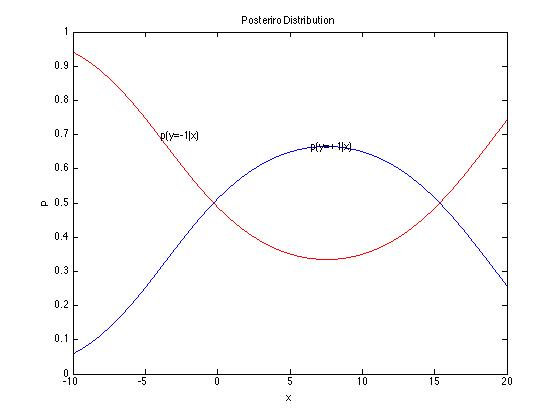
\includegraphics[width = 5in]{figure5.jpg}
\caption{Posteriro distribution}
\label{fig:5}
\end{figure}

To draw the ROC curve, we need hit rate which is the positive input that has been classifed as positive, given by the cdf of $p(y=-1|x)$ at $T$, and false alarm, which is the negitive that has been classified as positive, given by the cdf of $p(y=+1|x)$ at $T$. Then we can draw the picture at each T having the hit rate and false alarm, shown in figure \ref{fig:3}.

To draw the PR curve, we need TP, which is the decision that classify positive to positive, given by the cdf of $p(y=-1|x)$ at $T$; FP, which is the decision that classify negitive to positive, givne by the cdf of $p(y=+1|x)$ at $T$; FN, which is the decision that classify positive to negitive, given by integrate from $T$ to $+\infty$. Then precision is given by $TP/(TP+FP)$ and recall is given by $TP/(TP+FN)$. Then we could draw at each $T$, shown in figure \ref{fig:4}.
\begin{figure}
\centering
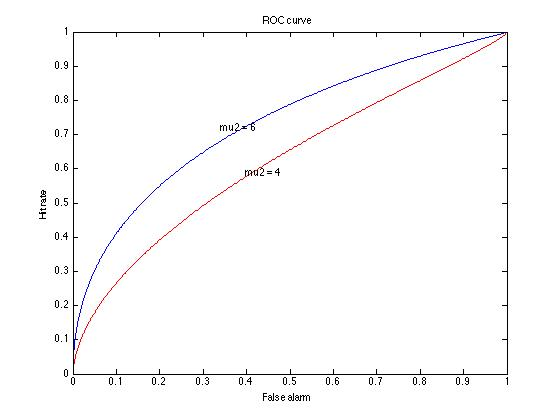
\includegraphics[width=5in]{figure3.jpg}
\caption{ROC curve}
\label{fig:3}

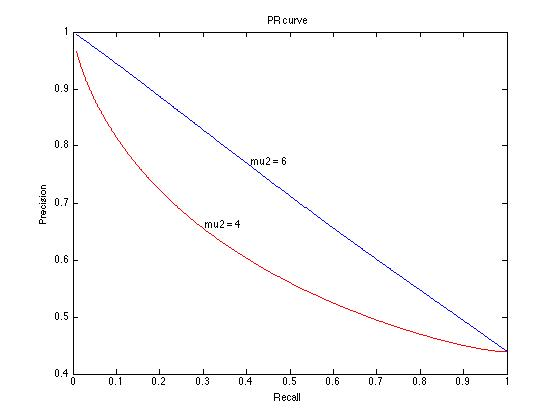
\includegraphics[width=5in]{figure4.jpg}
\caption{PR curve}
\label{fig:4}
\end{figure}

\item When we change $\mu_{2}$ to $4$, both ROC and PR would be worse, this is due to the fact that the two distribution become closer and there are more overlaps, and according to textbook, discriminability is defined as $d^{'} = \frac{|\mu_{2}-\mu_{1}|}{\sigma}$, and a higher $d^{'}$ is desirable.
\end{enumerate}

\end{document}